\chapter{Db2graph}
\label{chap:db2graph}

Im Rahmen dieses Kapitels wird IBM Db2graph genauer erläutert. Dabei wird der Ansatz, das Konzept und die bereits in der Dokumentation der Software beschriebenen Einschränkungen eingegangen. 

\section{Ansatz}
\label{db2graph:ansatz}
Db2graph wurde mit dem Ziel entwickelt, Informationen mittels Graph-Queries aus einer relationalen Db2 Datenbank abfragen zu können. So wurde Db2graph als eine Art Graph-Erweiterung für Db2 konzipiert. Der Einsatz von Db2graph setzt folglich eine aktive Instanz von Db2 voraus. Diese hält hierbei die Informationen, auf die Db2graph Zugriff hat, in relationaler Form. Dabei müssen die Daten nicht für die Einbindung in Db2graph angepasst werden.

\begin{figure}[h]
    \centering
    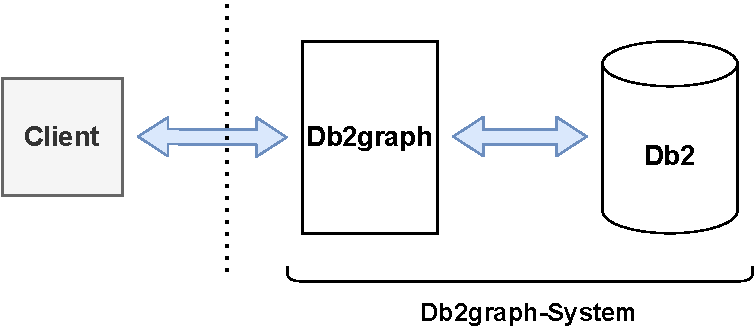
\includegraphics[width=\textwidth]{images/db2graph_system.pdf}
    \vspace{0.1em}
    \caption{Struktur Db2graph-System}
    \label{fig:db2graph_system}
\end{figure}

Wie in \autoref{fig:db2graph_system} erkennbar, fungiert Db2graph aus architektonischer Sicht als eine Art Proxy-Anwendung beziehungsweise Graph-Erweiterung für Db2. Dabei übersetzt sie die von einem Client gesendeten Gremlin-Graph-Queries in SQL-An\-wei\-sung\-en und leitet diese anschließend an eine Db2 Instanz weiter. Darüber hinaus können Db2 und Db2graph zusammengefasst als eine Art Hybrides Datenbankmanagementsystem betrachtet werden. Da es Elemente von Graph- und relationalen Datenbanksystemen vereint. So ist es möglich Graph-Anfragen an ein solches System zu stellen, während dem die Daten in relationaler Form gespeichert werden. Im weiteren Verlauf der Arbeit wird die Kombination aus Db2 und Db2graph verkürzt als Db2graph-System bezeichnet, wie bereits in \autoref{fig:db2graph_system} dargestellt. 

\section{Aufbau}
Wie in \autoref{fig:db2graph_aufbau} beschrieben, handelt es sich bei Db2graph um eine modular aufgebaute Anwendung. Die Anwendung besteht dabei aus fünf größeren Komponenten, siehe \autoref{fig:db2graph_aufbau}. Die fünf Komponenten übernehmen dabei die folgenden Rollen und Aufgaben: 

\begin{itemize}
    \item \textbf{TinkerPop-Stack}\\Stellt das Grundgerüst für Db2graph dar. Er parsed eingehende Gremlin-Queries und erstellt auf Basis dessen einen Query-Plan bzw. Abfrage-Plan \cite{vldb_tian}. Dabei interagiert er über API-Aufrufe mit den anderen Modulen \cite{vldb_tian}.
    \item \textbf{Topology}\\Beinhaltet die Funktionalität für das Mapping von relationalen Tabellen auf eine Graph-Struktur \cite{vldb_tian}, \cite{sigmod_tian}.
    \item \textbf{Graph Structure}\\Hierbei handelt es sich um eine eigene Implementierung einer Graph-Struktur auf deren Basis TinkerPop arbeitet \cite{vldb_tian}. Eine Implementierung dieser Struktur wird benötigt, um den vom TinkerPop-Stack erstellten Query-Plan durchzuführen \cite{sigmod_tian}. 
    \item \textbf{SQL-Dialect}\\Diese Komponente stellt die Funktionalität für die Erzeugung von Db2-kompatiblen SQL-Anweisungen bereit \cite{sigmod_tian}.
    \item \textbf{Traversal-Strategy}\\Dieses Modul stellt dem TinkerPop-Stack optimierte Traversal-Strategies zur Verfügung. Diese werden eingesetzt, um einen vom TinkerPop-Stack aufgestellten Query-Plan zu optimieren, bevor dieser ausgeführt wird \cite{sigmod_tian}.  
\end{itemize}

So stellt also der TinkerPop-Stack den Kern von Db2graph dar. Die Topology-, Graph-Structure und SQL-Dialect-Komponente hingegen bieten Db2graph und Db2 spezifische Funktionalität, auf die der TinkerPop-Stack zugreifen kann. Das Traversal-Strategy-Modul stellt darüber hinaus dem TinkerPop-Stack, optimierte Traversal-Strategies zur Verfügung. Diese helfen dem TinkerPop-Stack dabei die Performance von Query-Plans zu verbessern.  

\begin{figure}[h]
    \centering
    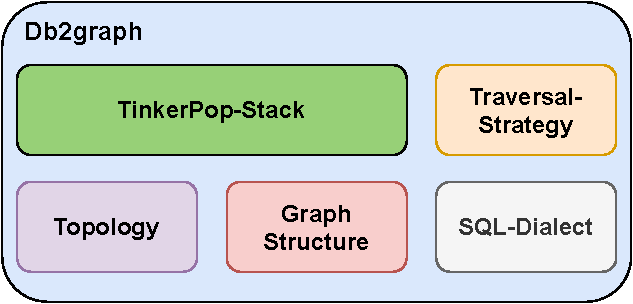
\includegraphics[width=\textwidth]{images/db2graph_components.pdf}
    \caption{Aufbau von Db2graph}
    \label{fig:db2graph_aufbau}
\end{figure}

\section{Funktionsweise}
\label{db2graph:funktionsweise}
Um die Funktionsweise von Db2graph genauer zu erläutern, wird in diesem Abschnitt die Funktionsweise aus verschiedenen Perspektiven erläutert. Im Rahmen der ersten Perspektive wird detailliert darauf eingegangen, wie ein Db2graph-System die Anfrage eines Clients verarbeitet. Bei der zweiten Perspektive handelt es sich hingegenum die Db2graph interne Perspektive. Im Zuge dessen wird beschrieben, wie eine Gremlin-Abfrage in Db2graph selbst als Anwendung verarbeitet wird. 

\section{Einschränkungen}
